\documentclass[./dissertation.tex]{subfiles}
\begin{document}


\chapter{Failure Mode and Effect Analysis FMEA}

\section{Introduction}
\subsection{General}
FMEA and FMECA are important techniques for a reliability assurance programme.They can be applied to a wide range of problems which may occur in technical systems, and can be carried out in varying degrees of depth, or modified, to suit a particular purpose. The analysis is carried out in a limited way during the conception, planning, and definition phases and more fully in the design and development phase. It is however important to remember that the FMEA is only part of a reliability and
maintainability programme which requires many different tasks and activities. FMEA is an inductive method of performing a qualitative system reliability or safety analysis from a low to a high level. A thorough understanding of the system under analysis is essential prior to undertaking FMEA. Functional diagrams and other system drawings are normally necessary for this understanding. Reliability block diagrams, fault trees and/or state diagrams are then usually derived from these in order to
carry out the analysis. In many instances the block diagram descriptions and block diagram failure descriptions are included in the FMEA format. Separate diagrarns will be needed for the
following:
\begin{enumerate}
    \item The way in which different criteria for system faiulre are determined;
    \item Degradation of function or reduction in assurance of function;
    \item Alternative operational phases
\end{enumerate}

\subsection{Purpose of the Analysis}
The reasons for undertaking FMEA (or FMECA) may include the following:

\begin{itemize}
    \item to identify those failures which have unwanted effects on system operation, e.g. safety critical failures;
    \item to satisfy contractual conditions that an FMEA should be completed;
    \item where appropriate, to quantify the reliability and/or safety of the system;
    \item to allow improvements of the system's reliability and/or safety (e.g. by design or quality assurance action)
    \item to produce aids to fault diagnosis;
    \item to allow improvement of the system's maintâinability (by highlighting areas of risk or non-conformance for maintainability).
\end{itemize}

ln view of these reasons the objectives of an FMEA (or FMECA) may include the following: 

\begin{enumerate}
    \item a comprehensive identification and evaluation of all the unwanted effects within the defined boundaries of the system being analysed, and the sequences of events brought about by each identified item failure mode, from whatever cause, at various levels of the system's functional hierarchy;
    \item the determination of the significance (or criticality) of each failure mode with respect to the system's correct function or performance and the impact on the reliability and/or safety of the process concerned;
    \item a classification of identified failure modes according to relevant characteristics, including detectability, diagnosability, testability, item replaceability, compensating and operating provisions (repair, maintenance, logistics, etp.);
    \item an estimation of measures of the significance and probability of failure.
\end{enumerate}


\subsection{Basic Principles of FMEA}
The following concepts are essential to FMEA:

\begin{enumerate}
    \item breakdown of the system into 'elements';
    \item a diagram of the system's functional structure and identification of the various data which are needed to perform the FMEA;
    \item the failure mode concept (a part may have several failure modes or a failure mode may involve several parts);
    \item identification of new physical features or new requirements;
    \item the criticality concept and the measure to be used (if criticality analysis is required).
\end{enumerate}

Further, it is essential to specify the existing links between the FMEA (and the FMECA) and other qualitative (and quantitative) analytical methods within the overall reliability programme.  Very few designs are wholly new. Most are to some extent developments of old designs. FMEA should use the information on existing systems and draw attention to the need for tests, etc. for the new parts.  



\section{Procedure}

\subsection{General}
The wide variation in complexity of system designs and applications may require the development of highly individualized FMEA procedures consistent with the information available. Traditionally, there have been wide variations in the manner in which FMEA is conducted and presented. However, the analysis is usually done in a standard manner and presented on a worksheet that contains a core of essential information which can be developed and extended to suit the particular system or project to which it is applied. A typical example of a worksheet is shown in Figure 1.

The procedure consists of the following four main stages:

\begin{enumerate}
\item Preparatory definition of the system including the design, functional, operational, maintenance, and environmental requirements;
\item Establishment of the basic principles and purposes of the FMEA and the form of its presentation;
\item Carrying out the FMEA using the appropriate worksheet designed according to (a) and (b);
\item Reporting of the complete analysis including any conclusions and recommendations made.
\end{enumerate}

A more detailed consideration of the information needed is given in Section 2.4.2.

\subsection{Preparation}
At the commencement of an analysis, the following preparations should be made:
\begin{enumerate}
\item The analyst should have available the information listed in Section 2.4.2.2 to 2.4.2.7 that clearly defines the system to be analyzed.
\item It will usually be necessary for the analyst to translate the information into some form of functional, hierarchical, or reliability block diagrams. An example of a functional diagram is shown in Figure 2. This diagram shows how the failure effects at the part level form the failure modes at the module level, the failure effects at the module level form the failure modes at the subsystem level, and so on. Such a representation of the system should explicitly identify the system's functional structure, the system boundary, and the inputs and outputs crossing that boundary. Further information is given in Section 2.4.2.8 to 2.4.2.10.
\end{enumerate}

\subsection{FMEA principles}
The following principles should be applied:
\begin{enumerate}
\item Define clearly the purposes and uses of the FMEA as indicated in Section 2.1.2.
\item Establish and define the relationships with other forms of reliability analysis with which the FMEA may subsequently be integrated. (See Section 2.3.5.)
\item Define the scope of the FMEA in relation to the functional structure and hierarchical structure of the system as described by the block diagrams referred to in Section 2.4.2.10. It is essential to define the lowest level in the system's hierarchical structure at which the analysis will start. The guidance given in Sections 2.3.4, 2.4.1, and 2.4.2.8 is especially important for this task.
\item Define the format of the FMEA worksheet to suit the project requirements. The core information considered essential is as follows:
\end{enumerate}

\begin{enumerate}
\item The name of the item in the system being analyzed;
\item Function performed by the item;
\item Identification number of the item;
\item Failure modes of the item;
\item Failure causes;
\item Failure effects on the system;
\item Failure detection methods;
\item Compensating provisions;
\item Severity of effects;
\item Remarks.
\end{enumerate}
Other information required for the particular system and project needs to be defined by the analyst according to the purposes of the



\section{Analysis}
It is worth to underline that, even though the scope of this thesis is to establish a new methodologyfor automated FMEA in both hardware and software systems, there is the absolute need to comply with what is today the state of the art for FMEA and the guidelines to be followed to bring the metrics extracted during the analysis to certification. It is for this reason that the following section will present the traditional method applied today to all the electromechanical systems under evaluation. Bare in mind that the totality of the procedure described below is man driven.

The usual requirement and purpose of an FMEA isto identify the effect of oJl failure modes of allconstituent items at the lowest level in the system.Tb achieve this the worksheet should be used inthe following manner:

\begin{enumerate}

	\item Identify all items in the system or subsystem,each of which is to have its failure modes andeffects analysed. The system of identification byname and number should be such that no itemswill be omitted.
	\item Select the first item for analysis and enter theitem name and identification number in theappropriate columns of the worksheet.Determine the function of that item in thesystem and enter that on the worksheet.
	\item Deduce all the possible failure modes of theitem due to any possible cause and individuallyenter these modes on the worksheet
	\item  Postulate the most likely failure causes foreach failure mode of the item and enter these onthe worksheet. It will usually not be possible to consider allpossible causes because the range is so vast, butthe most significant with regard to the item, thefailure mode and the application should beidentified.
	\item Deduce the effects of the failure on thesubsystem and system, as determined by thescope of the FMEA
	\item  Complete the remaining columns of theworksheet for the first failure mode of the firstitem.
	\item Repeat 3 to 5 for all failure moides of the first item
	\item Repeat 2 to 6 for all other items
\end{enumerate}


\subsection{Multiple Stages}
If the FMEA is to be done in stages that eachrelate to separate Ievels in the system's hierarchicalstructure, the failure effects from the lower level become the failure modes at the next level up. The analysis should then proceed as follows.

\begin{enumerate}
	\item Identify the lower level FMEAs that areappropriate for the next stage in the systemFMEA according to the system's hierarchicalstructure defined by the block or functionaldiagrams (see 2.2,2(b)). Where appropriate alsoinclude items defined as being at the lowest levelin that part of the system structure
	\item Perform the FMEA for each failure of eachitem at this higtrer level in the system stmctureas given in the previous section.
	\item repeat the two above steps for any further higher levels in the system structure.
\end{enumerate}
\subsection{Worksheet reccomendations}

The last worksheet entry should give any pertinent remarks to clarify other entries. Possible future actions such as recommendations for design improvements may be recorded and then amplified in the report. This column may also include the following:

\begin{enumerate}
\item[(a)] any unusual conditions;
\item[(b)] effects of redundant element failures;
\item[(c)] recognition of specially critical design features;
\item[(d)] any remarks to amplify the entry;
\item[(e)] references to other entries for sequential failure analysis;
\item[(f)] significant maintenance requirements;
\item[(g)] dominant failure causes;
\item[(h)] dominant failure effects;
\item[(i)] decisions taken, e.g. at design review.
\end{enumerate}


The report on the FMEA (or FMECA) may be included in a wider study or may stand alone. In neither case, the report should include a summary and a detailed record of the analysis and the block or functional diagrams which define the system structure. The report should also contain a list of the drawings (including issue status) on which the FMEA is based.

The summary should contain a brief description of the method of analysis and the level to which it was conducted, the assumptions and the ground rules. In addition, it should include listings of the following:

\begin{enumerate}
\item recommendations for the attention of designers, maintenance staff, planners, and users;
\item failures which, when initially occurring alone, result in serious effects;
\item failures which have no effect;
\item design changes which have already been incorporated as a result of the FMEA (or FMECA).
\end{enumerate}






\begin{figure}
	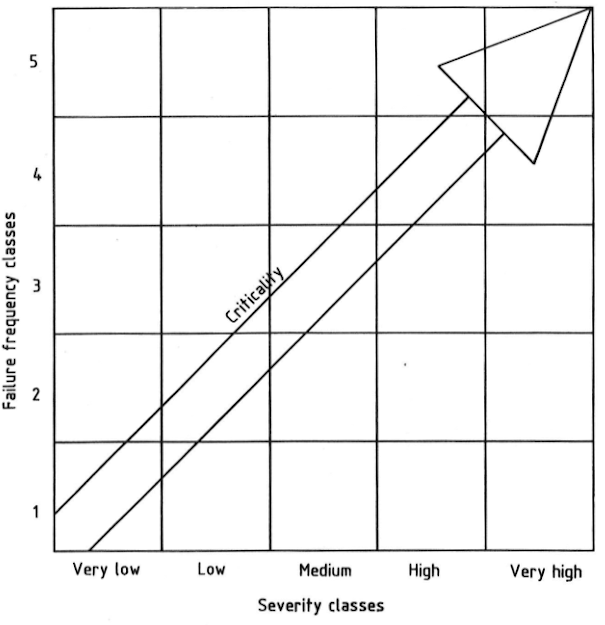
\includegraphics[width=\linewidth]{subfiles/imgs/fmea_criticality_grid.png}
  \caption{Criticality Grid}
	\label{fig:criticality_grid}
\end{figure}


\begin{figure}
	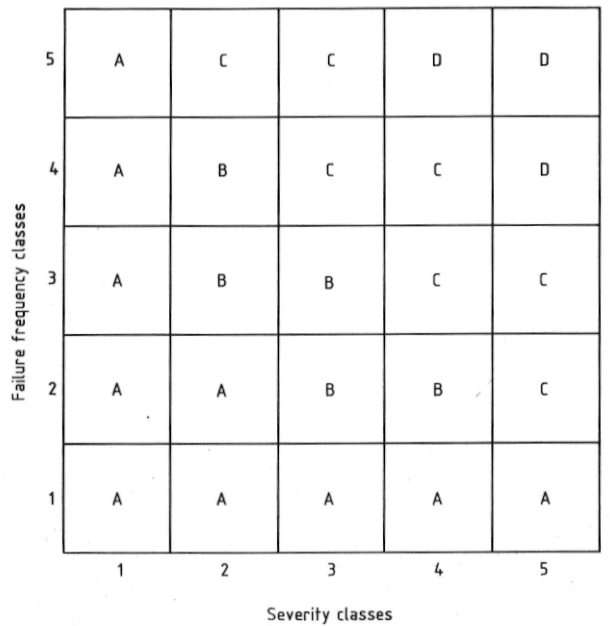
\includegraphics[width=\linewidth]{subfiles/imgs/fmea_criticality_matrix_with_bands.png}
  \caption{FMEA Criticality Matrix}
  \label{fig:criticality_matrix}
\end{figure}

\end{document}
